\chapter{Limite Continuo}

En esta seccion se va a estudiar la fucion $\zeta (s) $ en el limite $L \rightarrow \infty$, donde la funcíon $\zeta _A (s)$ va a quedar definida por:

\begin{equation}
\zeta (s) = \int _{0} ^{\infty} \rho (x) \ \left( \frac{x}{\mu } \right) ^{-2 s} dx
\end{equation}

Donde la $\rho(x) $ es la densidad de autovalores, para llegar a esta representación se va a utilizar la forma como integral, donde el camino de intregración de está dado por la figura izquierda de (\ref{fig:contorno}). La parametrización usada fue:


\[
z(t) =  
	  \begin{cases} 
      t + i \epsilon  & x _0 \leq t \leq \infty \\
      t - i \epsilon  & x _0 \leq t \leq \infty \\
      x _0 + i t		  & - \epsilon \leq t \leq \epsilon
   \end{cases}
\]

De (\ref{larga}) se puede ver que $S1,S2 \rightarrow 1$ cuando $L \rightarrow \infty$, por lo tanto se va a utilizar $M ( \lambda)$ dada por (\ref{eq.completa}).\\



Dependiendo si se está arriba o abajo del eje real, va a existir un termino exponencialmente creciente/decreciente en el limite $L \rightarrow \infty$ proveniente de $e ^{i z t}$

La integral correspodiente a arriba del eje real es:

\begin{equation}
\begin{array}{c}
\frac{1}{2 \pi i} \int _{\infty} ^{t0} 
\partial _z
Log
\left(
\frac{e ^{-2 i z  L } e ^{- \frac{i \alpha}{2 \lambda} Log \left( 2 z  L \right) } }
	 {\Gamma \left( 1 + \frac{ \alpha}{2 i z } \right)} +
\frac{e ^{ \frac{i \alpha}{2 z } Log \left( 2 z  L \right)  } }{\Gamma \left( 1 - \frac{ \alpha}{2 i z } \right) }
\right) d z \\
z = i t + \epsilon 
\end{array}
\end{equation}

Sacando factor comun de modo de obtener un termino exponencialmente decrenciente adentro del logatirmo se obtiene:

\begin{equation}
\frac{1}{2 \pi i}  \int _{\infty} ^{t0} 
\partial _{z}
\left(
\frac{i\alpha}{2 z} Log ( 2 z L ) - 
Log \left( \Gamma \left( 1 - \frac{ \alpha}{2 i z} \right) \right) +
Log \left( 1- \epsilon _L \right)
\right)
d z
\end{equation}

Donde $ \epsilon _L \rightarrow 0$ si $L \rightarrow \infty $ , utilizando el mismo razonamiento para la integral de abajo, y luego tomando el limite $\epsilon \rightarrow 0$, se obtiene:

\begin{equation}
\begin{array}{c}
\zeta (s) = 
\frac{L}{\pi}
\int _ {x_0} ^{\infty} x ^{-2s} dx + \\[10pt]
\frac{\alpha}{2 \pi } \int _{x_0} ^{\infty} 
\left(-
\frac{1}{ x ^2} +
\frac{Log \left( 2 x L \right) }{x ^2}  -
\frac{1}{ x ^2 } 
\left(
\psi (1 + \frac{i \alpha}{2 x}) + \psi (1 - \frac{i \alpha}{2 x}) 
\right)
\right)
x ^{-2s} d x
\end{array}
\end{equation}



Relizando las integrales termino a termino se obtiene:
\begin{equation}
\begin{array}{c}
\zeta (s) = 


\frac{L}{2 \pi} \frac{x _0 ^{1-2s}}{s-1/2} + 


\frac{\alpha}{2 \pi} x _{0} ^{-2s-1}
\left( 
	-\frac{1}{1+2s} +
	\frac{1}{(1+2s) ^2} +
	\frac{Log(2 L x _0)}{1+2s} 
	\right) + 

  \\[10pt]


- \frac{\alpha}{2 \pi}
\int _{x_0} ^{\infty} 
\left(
\psi(1 + \frac{i \alpha}{2 x}) +
\psi(1 - \frac{i \alpha}{2 x} )
\right)
x ^{-2s-2}
dx
\end{array}
\end{equation}


Para calcular el ultimo termino hay distintos desarrollos en serie de la funcion $\psi $ que se pueden usar, se va a usar el desarrollo dado en \cite{Abramowitz:1974:HMF:1098650}.

\begin{equation}
\begin{array}{cc}
\psi (1+ z ) = - \gamma + \sum _{n=2} ^{\infty} (-1) ^n \zeta (n) z ^{n-1} & |z| < 1
\end{array}
\end{equation}

El cual su radio de convergencia esta centrado alrededor de $x = 0$


El último termino queda expresado como:

\begin{equation}
\frac{\alpha}{2 \pi}
\int _{x_0} ^{\infty}
\left(
-2 \gamma -
2 \sum _{n=1} ^{\infty}
\zeta (2n+1) (-1) ^{n}
\left( \frac{\alpha}{2 x} \right) ^{2n}
\right)
x ^{-2s-2} dx
\end{equation}

Quedando la funcion $\zeta _A (s) $ :

\begin{equation}
\begin{array}{c}
\zeta _A (s) = 
\frac{L x0 ^{-2s+1} }{2 \pi } \frac{1}{s- 1/2} + 
\frac{\alpha x0 ^{-2s-1} }{8 \pi } \frac{1}{(s+1/2) ^2} + \\
\frac{\alpha x0 ^{-2s-1} }{4 \pi } 
\left(
Log[2 L x_0] + \gamma - 1
\right)
\frac{1}{s+1/2} + \\
\frac{x_0 ^{-2s}}{2\pi} 
\sum _{n=1} ^{\infty} (-1) ^{n} \zeta (2n+1) 
( \frac{\alpha}{2 x0} ) ^{2n+1} \frac{1}{s+n+1/2}
\end{array}
\end{equation}

Para ver la energía de vacío hay que evaluar esta expresion en $s=-1/2$ y graficar su parte finita, tal como esta en la figura [ \ref{fig:vacio} ] donde estan los primeros 100 terminos de la serie, en funcion de $x = \alpha / x_0$ y la suma exacta de la serie al reemplazar $\zeta (2s+1) = 1$.

\begin{figure}
    \centering
    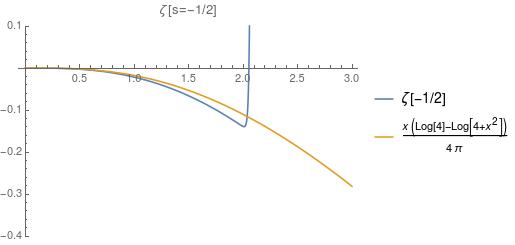
\includegraphics[scale=0.3]{Vacio.jpg}
    \caption{En esta imagen esta graficada la parte finita de la $\zeta _A (-1/2) $ en funcion del parametro $x= \frac{\alpha}{x _0}$ donde se sumaron los primeros 100 terminos de la serie, y en azul se puede ver la suma de la serie al reemplazar $\zeta (2n+1) = 1$}
    \label{fig:vacio}
\end{figure}